% The Stochastic Queue p-Median Problem
% O. Berman, R.C. Larson, C. Parkan 
% 1987
\subsection{Improvement}
\begin{frame}
This problem is presented by Berman et. al in \cite{berman1987stochastic}

\begin{itemize}
\item $G(N,L)$ the transportation network
\item $N$ the set of demand centers, with $|N| = n$
\item $L$ the set of all transportation arteries, the links
\item $h_j$ the fraction of service calls associated with each node $j$
\item $d(X,Y)$ is the shortest path between any two points $X,Y \in G$
\item $p$ number of response units
\item $\bar{X}$ the home locations of the service units while available
\item $\lambda$ mean rate per unit of time within service calls are generated in Poisson manner
\end{itemize}
\end{frame}

\begin{frame}
Given the arrival of a call for service,
exactly one of the servers is dispatched to it 
assuming that at least one server is available.

The service time for any service unit \textit{i}
is the sum of two components:
\begin{itemize}
\item The non-travel time component, 
  which is the sum of on-scene and off-scene service time.
\item Travel time component, which is the sum of travel time
  to the location of the call and travel time back to the home location.
\end{itemize}
\end{frame}

\begin{frame}
The mean service time for a service unit located at $\bar{X}^i$ is denoted $S(\bar{X}^i)$,
\begin{equation}
  S(\bar{X}^i) = \sum_{j = 1}^{n}{h_j^i\left(\bar{W}_{ij}+\frac{{\beta}_i}{v_i}d(\bar{X}^i,j)\right)} \; i=1,\ldots,p
\end{equation}
\begin{itemize}
\item $\bar{W}_{ij}$ is the mean of the \textbf{non-travel time} component $W_{ij}$
\item $v_i$ is the \textbf{travel speed} of unit \textit{i} to the scene of the call which is assumed constant
\item $\beta_i$ is a constant that allows different travel speeds to and from the scene of the call
\item $h_j^i$ is the probability that server \textit{i} is dispatched to node \textit{j} given that server \textit{i} is dispatched to a call for service.
\end{itemize}
\end{frame}

\begin{frame}
Whenever a call for service arrives while at least one of the servers is free at its home location,
the closest available server to the call will be dispatched.
Calls that find all servers busy enter a queue.
The queue discipline is assumed to be First-Come-First-Served.
The expected response time to a random call denoted by $\bar{T}_R(X)$ is the sum of two components
\begin{equation*}
  \bar{T}_R(\bar{X}) = \bar{W}_q(\bar{X})+\bar{t}(\bar{X})
\end{equation*}

\begin{itemize}
\item $\bar{W}_q(\bar{X})$ is the expected \textbf{waiting time} in the queue
\item $\bar{t}(\bar{X})$ is the expected \textbf{travel time} to the call.
\end{itemize}

The objective is to find a set of \textit{p} locations $\bar{X}^*$ on the network such that
\begin{equation*}
  \bar{T}_R(\bar{X}^*) \leq \bar{T}_R(\bar{X}) \; \forall \bar{X} \in G
\end{equation*}

$\bar{X}^*$ is called \textbf{the stochastic queue p-median}.
\end{frame}

\frame{\begin{figure}[h!]\centering{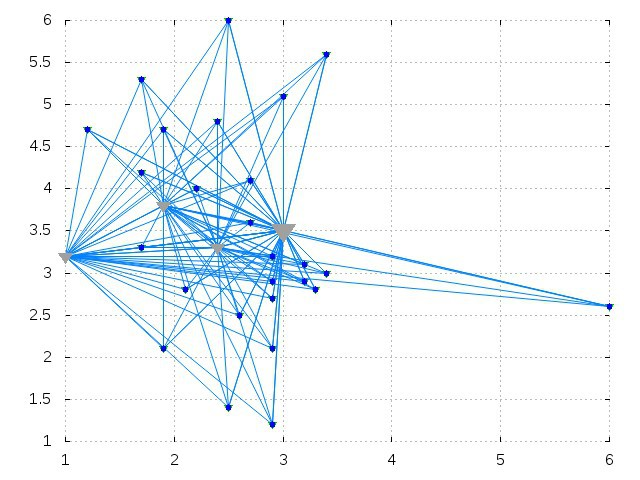
\includegraphics[scale=0.45]{SQM_Heuristic_1}\caption{m = n = 30, p = 5, iteration = 1}}\end{figure}}
\frame{\begin{figure}[h!]\centering{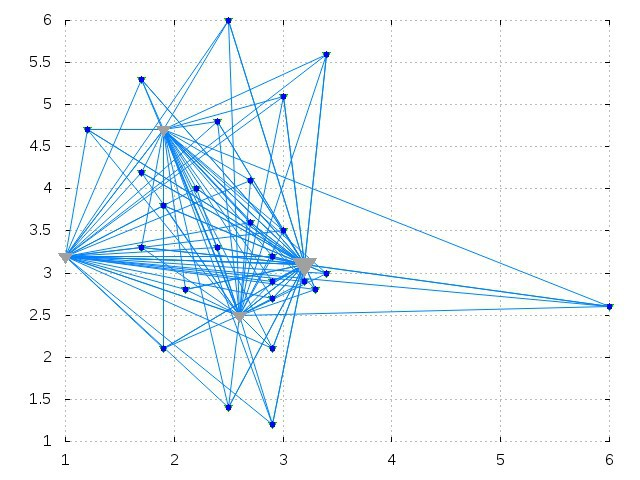
\includegraphics[scale=0.45]{SQM_Heuristic_2}\caption{m = n = 30, p = 5, iteration = 2}}\end{figure}}
\frame{\begin{figure}[h!]\centering{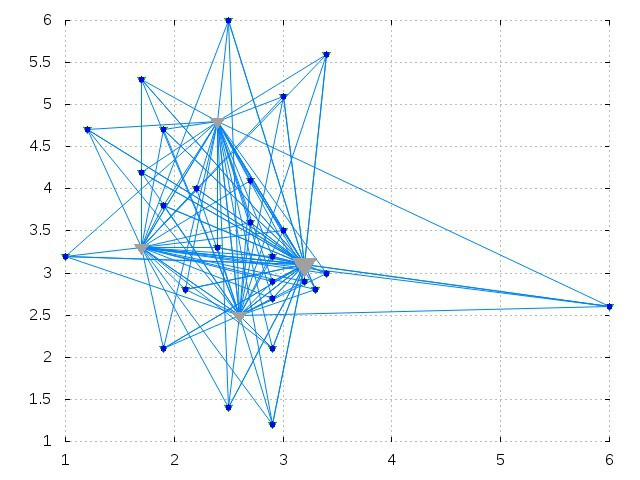
\includegraphics[scale=0.45]{SQM_Heuristic_3}\caption{m = n = 30, p = 5, iteration = 3}}\end{figure}}
\frame{\begin{figure}[h!]\centering{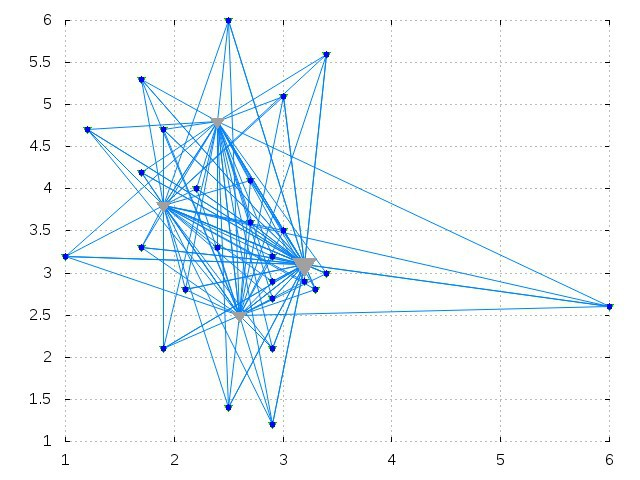
\includegraphics[scale=0.45]{SQM_Heuristic_4}\caption{m = n = 30, p = 5, iteration = 4}}\end{figure}}
